\chapter{Marco teórico}
\label{Marco_teorico}

\section{Estudio de mercado}
A lo largo de los años los \ac{RTS} siempre han contado con una gran aceptación entre
los usuarios de \ac{PC}, un claro ejemplo de esto puede ser el juego \textit{`Age of
Empire II: The Age of Kings'}\footnote{Desarrollado por `Ensemble Studios' y lanzado a
finales de 1999.} el cual se posicionó como uno de los juegos más vendidos del momento
superando el millón de copias. Actualmente el juego cuenta con una remasterización
\footnote{Co-desarrollado por Forgotten Empires, Tantalus Media y Wicked
Witch. Lanzado en noviembre de 2019.} la cual ha conseguido vender más de 50.000
copias en \textit{`Steam'}.

Si miramos en el panoráma nacional, podemos encontar el juego \textit{`They Are
Billions'} \footnote{Desarollado por Numantian Games y lanzado en junio de 2019.}
disponible inicialmente para \ac{PC} y posteriormente lanzado en \textit{`PlayStation 4'}
y \textit{`Xbox One'} debido a su éxito. A día de hoy el juego a conseguido vender
solamente en \textit{`Steam'} más de 25.000 unidades con una valoración muy positiva por
parte del público.

El género puede aparentar ser cosa del pasado pero vistas las cifras podemos concluir
que sigue siendo un reclamo para los jugadores.

\section{Referentes}
A la hora de establecer las mecánicas, el apartado artístico y/o otros aparatados del
juego es habitual basarse o tener en cuenta lo que han hecho otras entregas anteriores
en su momento. Para el desarrollo de este proyecto han sido de gran utilidad una
serie de entregas entre las que cabe destacar dos.

\subsection{Age of Empires II: The Age of Kings}
En primer lugar encontramos el juego \textit{'Age of Empires II: The Age of Kings'}, en
este juego tendremos que gestionar una civilizacion a elegir entre un amplio abanico de
facciones con sus propias unidades y edificaciones.

\begin{figure}[ht]
\centering
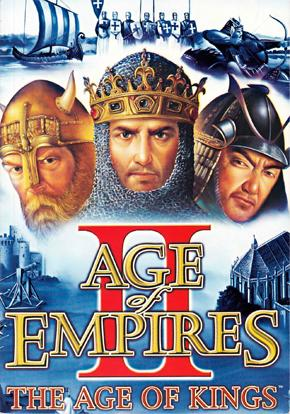
\includegraphics[width=0.5\textwidth]{imagenes/aoe_1.png}
\caption{Carátula del juego original.}
\label{img:aoe_1}
\end{figure}

El jugador deberá ser capaz de guiar a las unidades, gestionar las ciudades y conseguir
recursos a lo largo del escenario con el fin de derrotar a las demás facciones. Además se
nos presenta una serie de campañas en las cuales manejaremos a grandes personajes de la
historia como `William Wallace' o `Juana de Arco' entre otros.

Como podemos ver en la imágen~\ref{img:aoe_2}

\begin{figure}[ht]
\centering
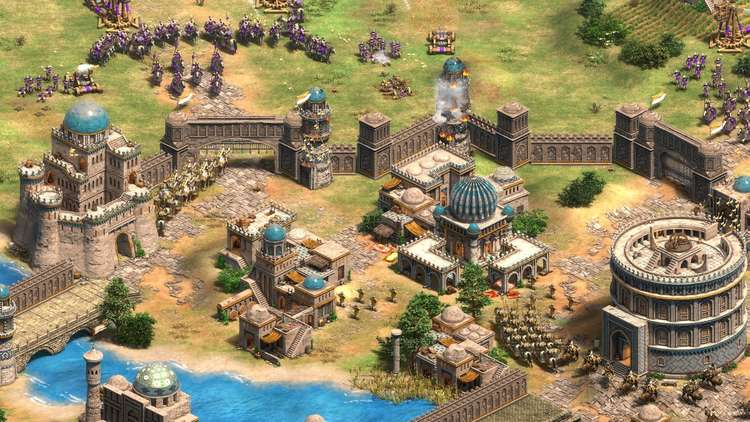
\includegraphics[width=0.5\textwidth]{imagenes/aoe_2.png}
\caption{Ciudad siendo asediada.}
\label{img:aoe_2}
\end{figure}

\subsection{The Are Billions}
yeee

\section{Algoritmos de IA}
yeee

